\section{Historical Development of Neural Networks}






\subsection{Mathematical Insight: Gradient Descent Connection}
The vectorized perceptron learning rule is actually a special case of gradient descent. The weight update \(\Delta W = \eta \cdot X^T \cdot E\) can be derived from minimizing the perceptron loss function:

\subsubsection{Loss Function}
For a single misclassified example, the perceptron loss is:
\[L = \max(0, -y_{\text{true}} \cdot z)\]
where \(z = \mathbf{w}^T \mathbf{x}\) is the net input.

\subsubsection{Gradient of the Loss}
The gradient with respect to weights is:
\[\frac{\partial L}{\partial \mathbf{w}} = -y_{\text{true}} \cdot \mathbf{x}\]
for misclassified examples, and 0 for correctly classified ones.

\subsubsection{Batch Update Rule}
For a batch of examples, the total gradient is:
\[\frac{\partial L_{\text{total}}}{\partial \mathbf{w}} = \sum_{i} \frac{\partial L_i}{\partial \mathbf{w}} = X^T \cdot (Y_{\text{pred}} - Y_{\text{true}})\]

This shows that our vectorized update rule \(\Delta W = \eta \cdot X^T \cdot E\) is exactly gradient descent with the perceptron loss function.

\subsection{Computational Complexity Analysis}
\subsubsection{Vectorized vs. Sequential Processing}
\begin{itemize}
    \item \textbf{Sequential}: \(O(m \cdot n)\) time for \(m\) examples and \(n\) features, but cannot leverage parallel hardware
    \item \textbf{Vectorized}: Same \(O(m \cdot n)\) time complexity, but:
    \begin{itemize}
        \item Can utilize SIMD (Single Instruction, Multiple Data) operations
        \item Reduces Python interpreter overhead
        \item Enables GPU acceleration for large matrices
        \item Better cache locality and memory access patterns
    \end{itemize}
\end{itemize}

\section{Geometric Interpretation of the Perceptron}
Understanding a Perceptron involves grasping the geometry of how it makes decisions. We can visualize this geometry in two primary ways: the \textbf{Input Space} and the \textbf{Weight Space}.

\subsection{Mathematical Foundation of Decision Boundaries}
The perceptron's decision boundary is defined by the hyperplane equation:
\[\mathbf{w}^T \mathbf{x} + b = 0\]



\subsubsection{Margin and Support}


\subsection{Example: The NOT Function}
\subsubsection{The Input Space}
The Input Space is a geometric representation of the data points. The goal of the Perceptron is to find a \textbf{decision boundary}---a line in 2D, or a hyperplane in higher dimensions---that perfectly separates the positive and negative data points.
\begin{figure}[h!]
\centering
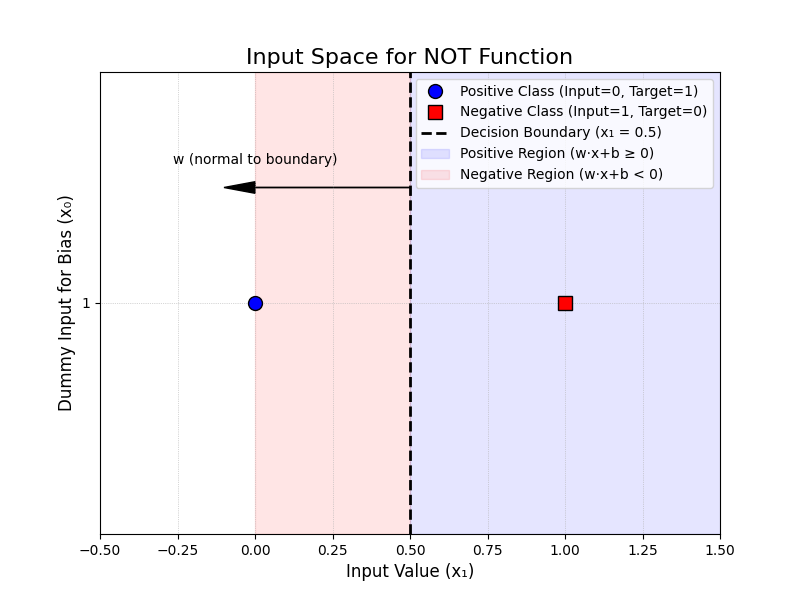
\includegraphics[width=0.6\textwidth]{not_input_space.png}
\caption{Input Space for the NOT Function.}
\end{figure}

\subsubsection{The Weight Space}
While the input space plots the data, the \textbf{Weight Space} plots the possible solutions. The axes of this space are the weights themselves. Every point in this space represents a different Perceptron model.
\begin{figure}[h!]
\centering
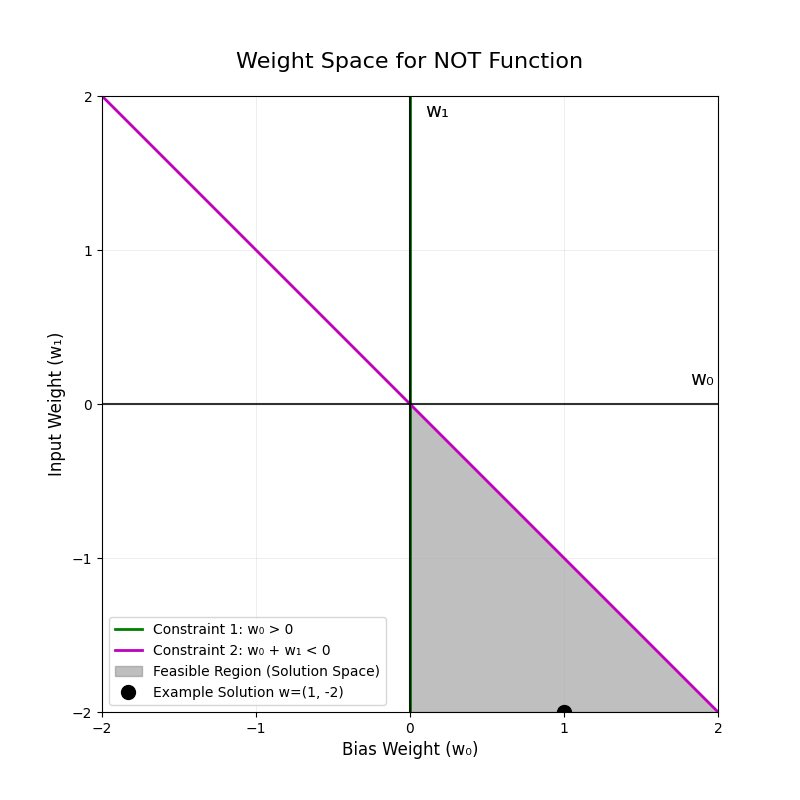
\includegraphics[width=0.6\textwidth]{not_weight_space.png}
\caption{Weight Space for the NOT Function.}
\end{figure}

\subsection{Example: The AND Function}
\subsubsection{The Input Space}
The Input Space shows our data points and the decision boundary that separates them. For the AND function, we have three "negative" points (target=0) and one "positive" point (target=1).
\begin{figure}[h!]
\centering
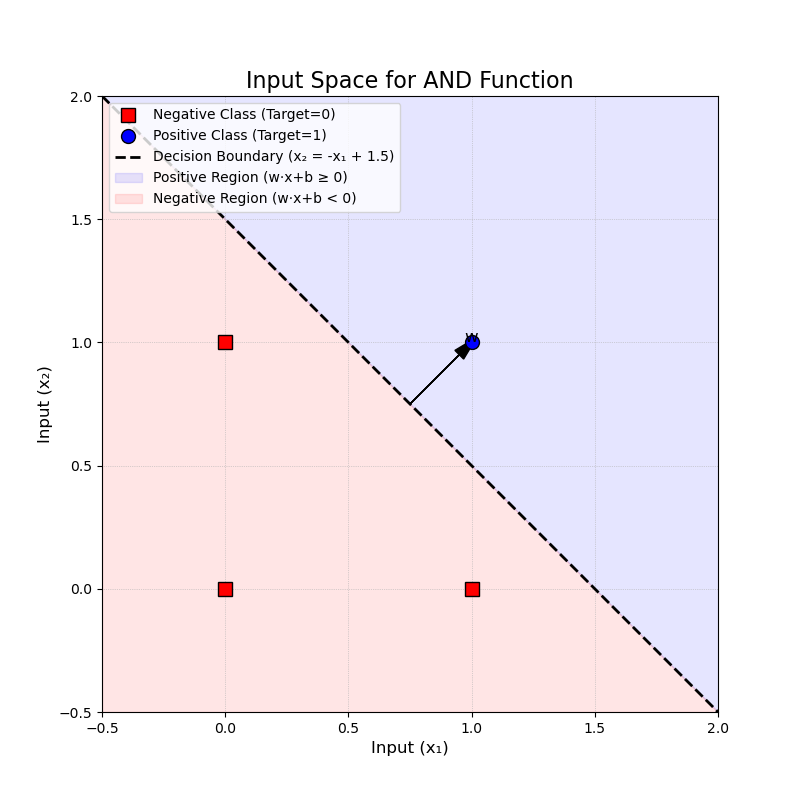
\includegraphics[width=0.6\textwidth]{and_input_space.png}
\caption{Input Space for the AND Function.}
\end{figure}

\subsubsection{The Weight Space}
The Weight Space represents the set of all possible solutions. Each of our four data points imposes a constraint on the possible values of the weights.
\begin{figure}[h!]
\centering
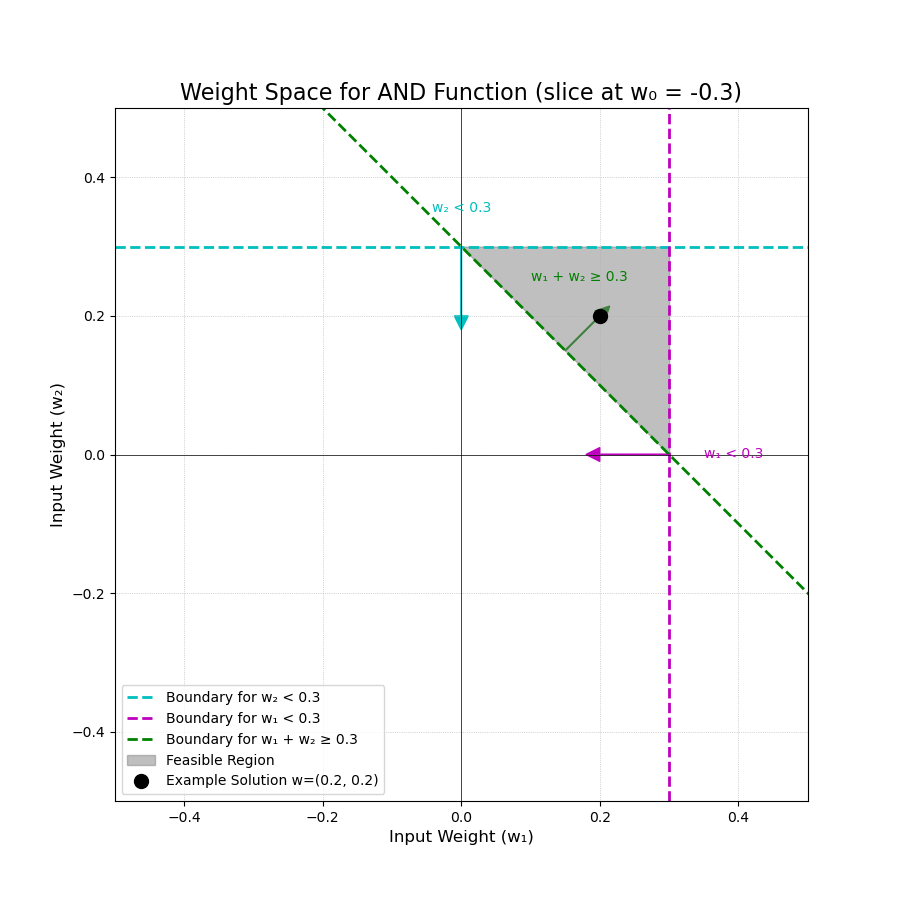
\includegraphics[width=0.6\textwidth]{and_weight_space.png}
\caption{A 2D slice of the Weight Space for the AND Function, with \(w_0 = -0.3\).}
\end{figure}


